\chapter{Apartado B: \textbf{Flujo Óptico}}
\label{chapter:tarea_b}

\section*{Tarea B.1: Configuración del Flujo Óptico}
\phantomsection
\addcontentsline{toc}{section}{Tarea B.1: Configuración del Flujo Óptico}
Para esta tarea vamos a utilizar el video \texttt{'slow\_traffic\_small.mp4'}. Para cargarlo utilice el método que se ha desarrollado anteriormente.
Implemente el flujo óptico de Lucas-Kanade, útil para detectar el movimiento pixel a pixel. Para ello vamos a comenzar por definir los parámetros necesarios para utilizar el método \texttt{cv2.calcOpticalFlowPyrLK}\footnote{ \href{https://docs.opencv.org/4.8.0/dc/d6b/group\_\_video\_\_track.html\#ga473e4b886d0bcc6b65831eb88ed93323}{Documentación del método Optical Flow Lucas-Kanade en OpenCV:} \\{https://docs.opencv.org/4.8.0/dc/d6b/group\_\_video\_\_track.html\#ga473e4b886d0bcc6b65831eb88ed93323}}

\section*{Tarea B.2: Detección de Puntos de Interés}
\phantomsection
\addcontentsline{toc}{section}{Tarea B.2: Detección de Puntos de Interés}
Configure los párametros para obtener los puntos de interés iniciales en el primer frame con el método de \texttt{cv2.goodFeaturesToTrack}\footnote{ \href{https://docs.opencv.org/4.8.0/dd/d1a/group\_\_imgproc\_\_feature.html\#ga1d6bb77486c8f92d79c8793ad995d541}{Documentación del método Shi-Tomasi en OpenCV:} \\{https://docs.opencv.org/4.8.0/dd/d1a/group\_\_imgproc\_\_feature.html\#ga1d6bb77486c8f92d79c8793ad995d541}}.

\section*{Tarea B.3: Cálculo y Visualización del Flujo Óptico}
\phantomsection
\addcontentsline{toc}{section}{Tarea B.3: Cálculo y Visualización del Flujo Óptico}
Calcule el flujo óptico con el método de Lucas-Kanade aplicando \texttt{cv2.calcOpticalFlowPyrLK} y visualice el movimiento de cada punto de interés en los siguientes frames.

\begin{figure}[H]
    \centering
    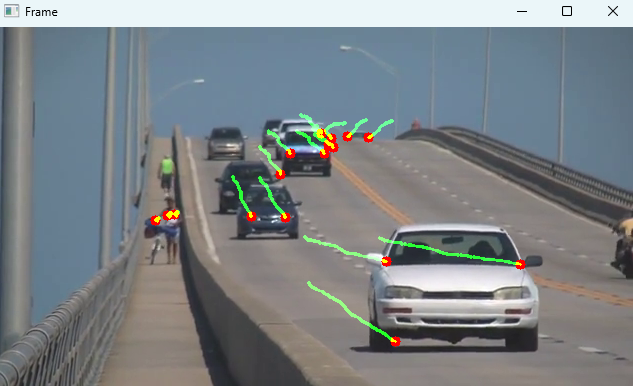
\includegraphics[width=0.45\textwidth]{Lab_4/template/figures/of_lk.png}
    \caption{Ejemplo de resultado de obtener el flujo ópitco con el metodo de Lucas-Kanade.}
    \label{fig:ejemplo_opticalflowLK}
\end{figure}

\section*{Preguntas}
\addcontentsline{toc}{section}{Preguntas}

\vspace{5mm}
\begin{tcolorbox}[colback=gray!10, colframe=gray!30, coltitle=black, title=Pregunta B.1, halign=left]
¿Qué efecto tiene el parámetro \texttt{winSize} en la precisión del flujo óptico?
\end{tcolorbox}


\vspace{5mm}
\begin{tcolorbox}[colback=gray!10, colframe=gray!30, coltitle=black, title=Pregunta B.2, halign=left]
¿Cómo influye el parámetro \texttt{qualityLevel} en la función \texttt{cv2.goodFeaturesToTrack} al detectar puntos de interés?
\end{tcolorbox}